\section{The search problem}
The Binary Search is a classical algorithm used to efficiently locate a hidden target element in a linearly ordered set. To do so, the searcher repeatedly picks the median element of such set, performs a comparison operation and in constant time learns if the target was found and if not, whether the target is above or below the median (For example see Figure \ref{fig:binary-search-subarrays}).


\begin{figure}[ht]
\centering
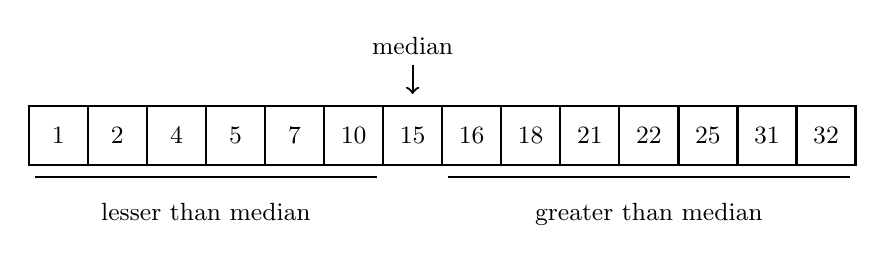
\begin{tikzpicture}[every node/.style={font=\small}, scale=0.75]

% --- Array values (10 elements) ---
\def\A{{1, 2, 4, 5, 7, 10, 15, 16, 18, 21, 22, 25, 31, 32}}
\def\MID{6} % Index of median (0-based): value = 23
% Draw array elements and indices
\foreach \i in {0,...,13} {
    \pgfmathsetmacro{\val}{\A[\i]}
    \draw[thick] (\i, 0) rectangle ++(1,1);
    \node at (\i+0.5, 0.5) {\val};
}

% Underline LEFT subarray (0..3)
\draw[thick] (0.1, -0.2) -- (6.0-0.1, -0.2);
% Label
\node[below=6pt] at (3, -0.2) {lesser than median};

% Underline RIGHT subarray (5..9)
\draw[thick] (7+0.1, -0.2) -- (13+1-0.1, -0.2);
% Label
\node[below=6pt] at (10.5, -0.2) {greater than median};

% Arrow for mid
\draw[<-, thick] (\MID+0.5, 1.2) -- +(0, 0.5) node[above] {median};

\end{tikzpicture}
\caption[Binary search]{Example of a sorted array containing 14 elements. }
\label{fig:binary-search-subarrays}
\end{figure}


The study of searching was initiated by D. Knuth in his seminal book \cite{Knuth1973} in which he discussed its various variants. However, the origins of the search problem reach the famous Rényi-Ulam game of twenty one questions in which a player is required to guess an unnamed object by asking yes-or-no questions\footnote{Note that in the twenty-one questions game one answer to a question may be a lie.}. Throughout the years, the searching and its variants have been continuously rediscovered under various definitions and names. This hints that the intuitions behind this problem resurface among multiple use cases and research domains. In fact, the search problem in its many variants is deeply connected with many other algorithmic notions including: parallelization of the Cholesky factorization, scheduling join operations in database queries, VLSI-layouts, learning theory, data clustering, graph cuts and parallel assembly of multi-part products. This work aims to serve as a survey of the results obtained for the problem and an experimental analysis of algorithms aimed at solving it.

The importance of searching is also due to its various practical applications. For example consider the following scenario: a complex procedure contains a hidden bug required to be fixed. The procedure is composed of multiple (often nested) blocks of code. In order to find this hidden bug the searcher can perform tests which allow him to check whether the given block of code contains the bug. After performing each such test they learn whether the bug is in or outside of the tested block. This process then continuous, until the bug is found. The problem is to find the best testing strategy for the tester in order to find the bug efficiently.

% A different scenario may occur in the medical diagnostics. The so called \textit{House M.D. Problem} is concerned with diagnosing a potentially lethal, hidden disease. In order to do so, House and his medical team perform series of tests on the patient. These tests (often avant-garde in their nature) may include blood tests, a family survey or even breaking into the patients house. After performing each such test the team learns some new information about the patient which allows them to iteratively narrow the size of the space of possible diagnoses. The outcome of such test may include for example: the sugar level in blood is low (or high), the patients mother died of a disease with similar symptoms, the patient consumes very large amount of tuna etc. As the condition of the patient is deteriorating rapidly, the team needs to determine the disease as quickly as possible. 

